\section{L-M ties}
Looking at the HR diagram we see that there appears to be a connection between mass and luminosity. We'll dwell on this for a while. This also connects to its life span and evolution. Observationally, if we plot the luminosity as a function of the mass, we find something that looks like this

\begin{figure}[!htb]
	\centering
	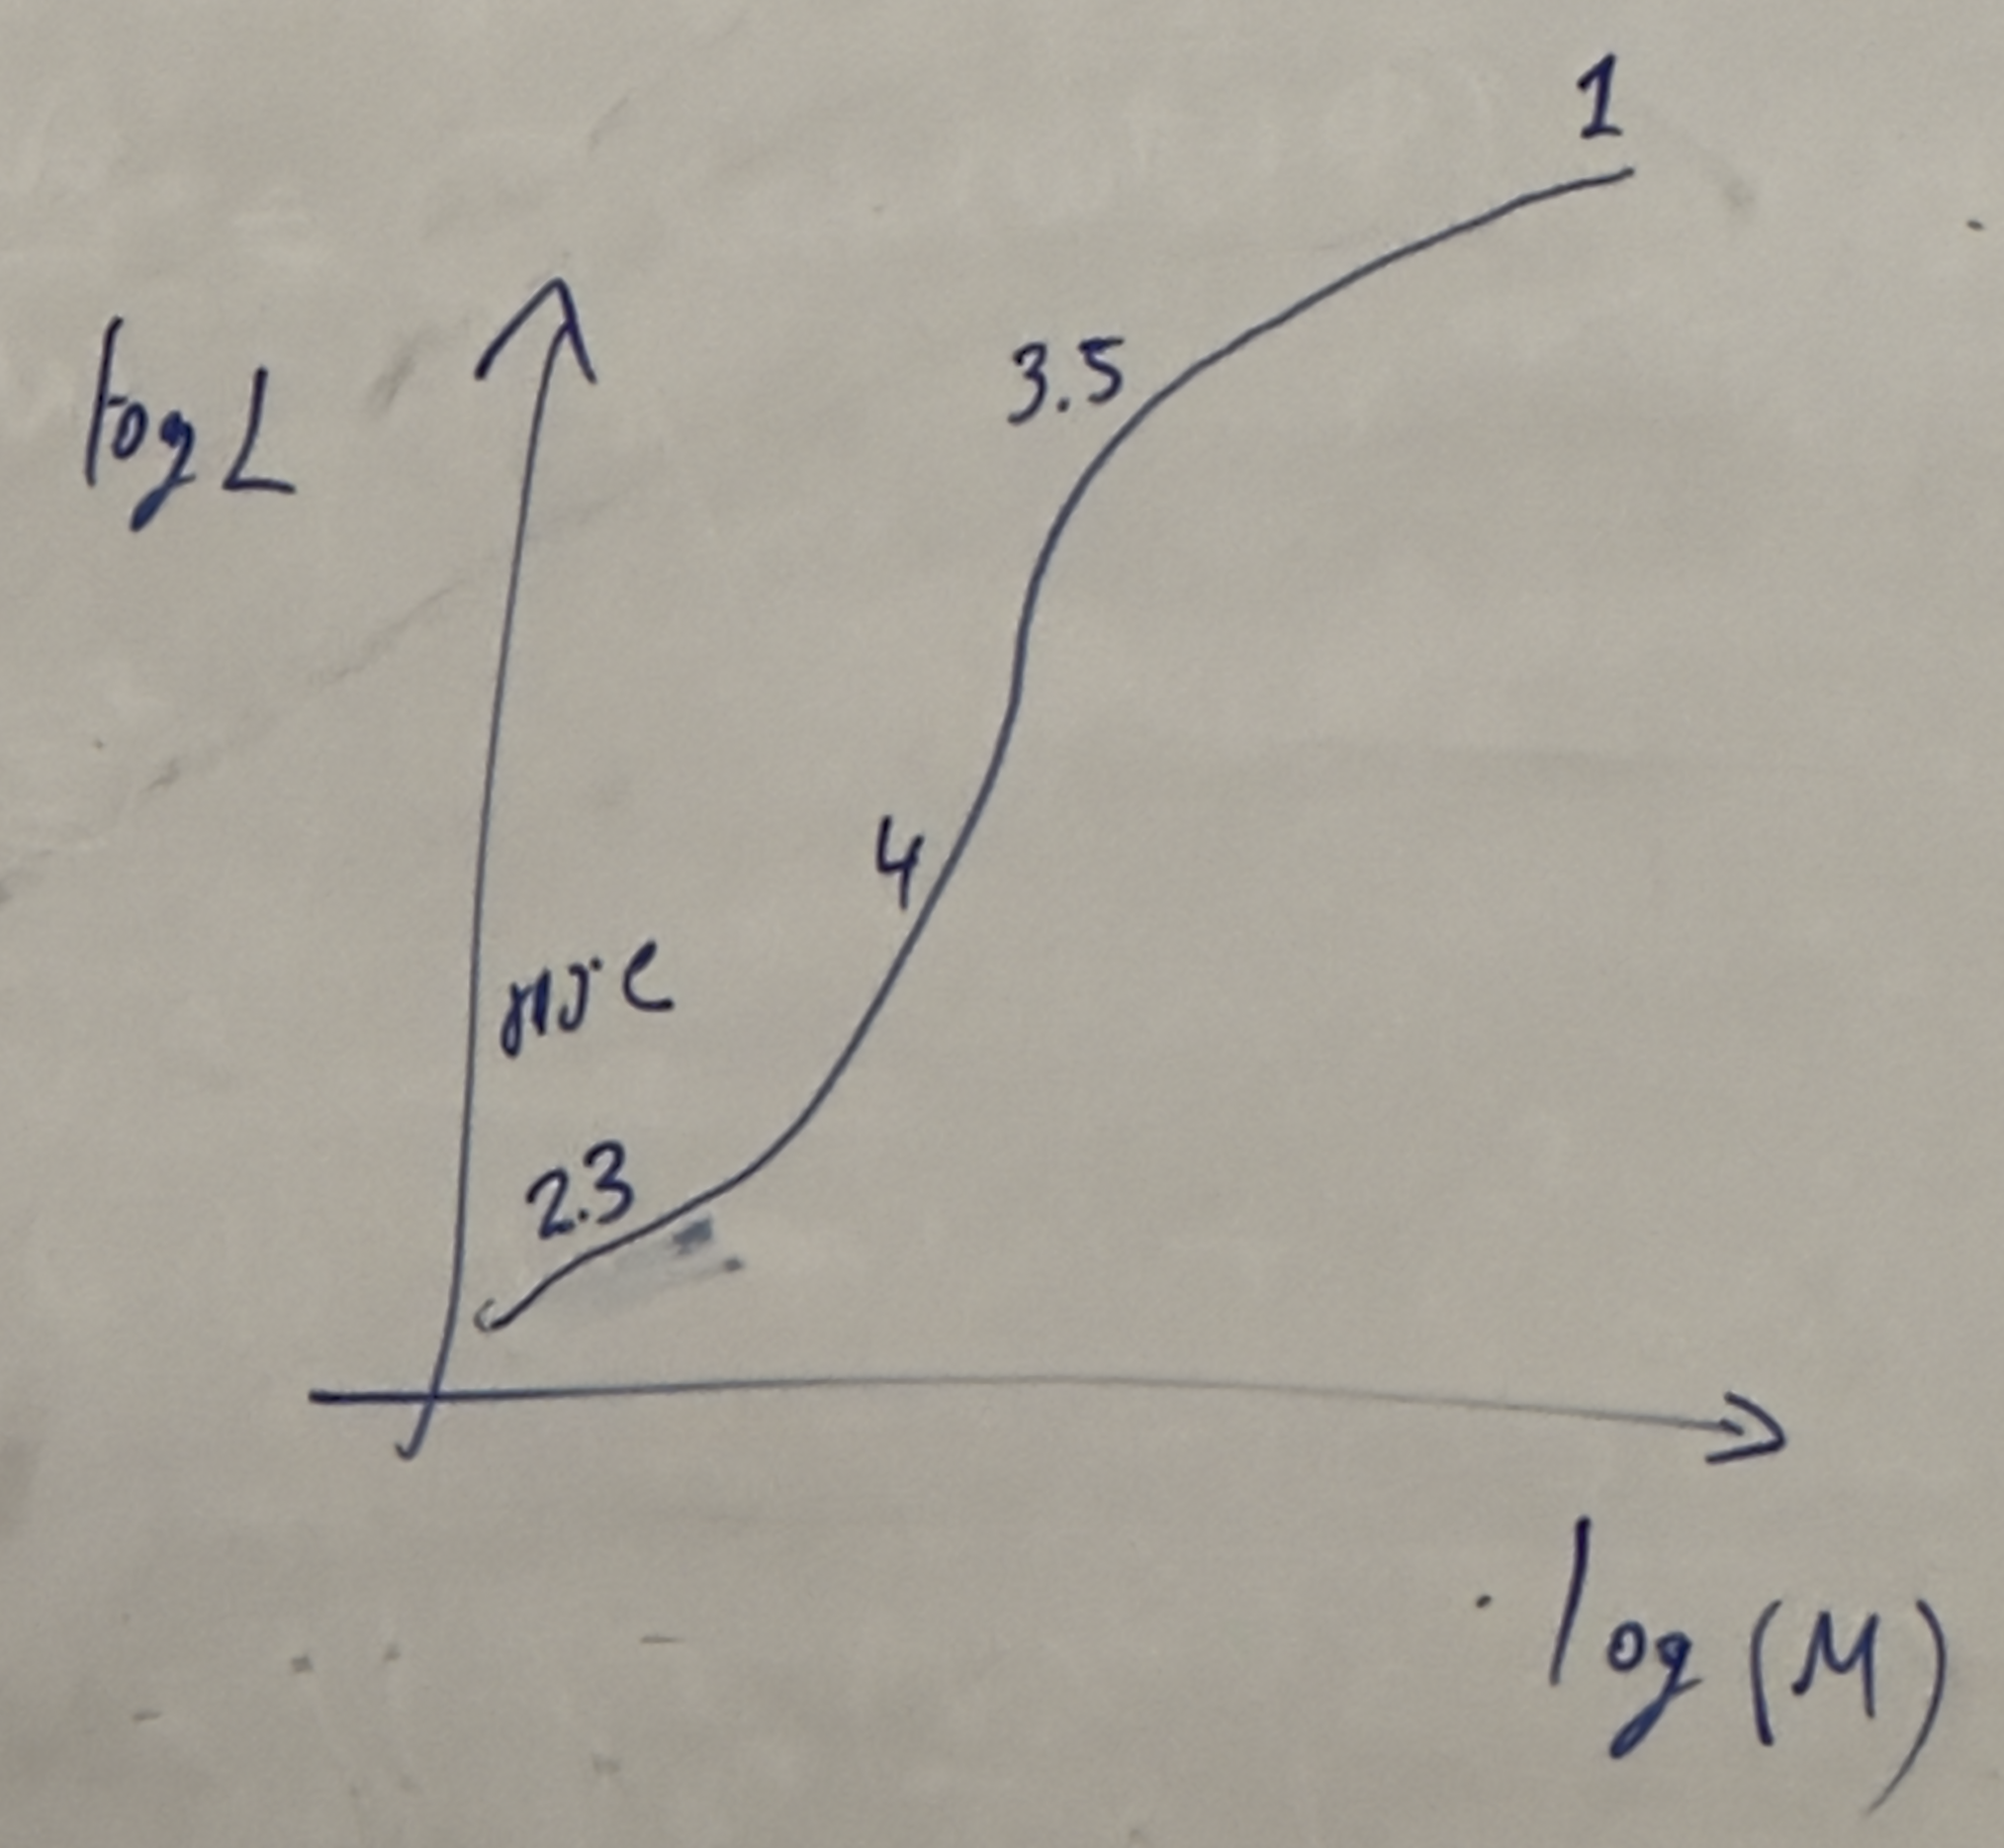
\includegraphics[width=0.75\textwidth]{images/IMG_0553.png}
	\caption{A diagram of the L-M relation}
\end{figure}

and using the relation
\begin{equation}
	\frac{L}{L_\mathSun} = A\ins{\frac{M}{M_\mathSun}}^\alpha
\end{equation}
we can write this as a table
\begin{table}[!htb]
	\centering
	\begin{tabular}{l|cc}
	  \(M/M_\mathSun \) & \(A\) & \(\alpha \) \\
	  \hline
	  \(<0.43\)& 0.23 & 2.3 \\
	  0.43--2 & 1 & 4\\
	  2--55 & 1.4 & 3.5\\
	  \(>55\) & \(\qty{3.2e4}{}\) & 1
	\end{tabular}
\end{table}
To get a feeling for why this behaves like this, we'll do the following. We'll assume
\begin{equation}
	\kappa = \kappa_{\text{Thomson}} = \text{const.}
\end{equation}
which is a good approximation for massive stars (2 to 55 solar masses). We'll also assume a power law of the form
\begin{align}
	M_r \propto r^\alpha && P \propto r^\beta && T \propto T^r
\end{align}
therefore the stellar structure equations become
\begin{align}
	\beta \frac{P}{r} \propto \frac{M\rho}{r^2} && \alpha\frac{M}{r} \propto r^2\rho && \gamma\frac{T}{r}\propto \frac{L\kappa\rho}{r^2T^3}
\end{align}
rearranging we find
\begin{align}
	P \propto \frac{M\rho}{r} && M\propto r^3\rho && L\propto\frac{T^4r}{\rho} && P \propto \rho T
\end{align}
Inserting D into A we find
\begin{equation}
	T \propto \frac{M}{r}
\end{equation}
and inserting that into C
\begin{equation}
	L\propto\frac{\ins{M/r}^4r}{\rho}=\frac{M^4/r^3}{\rho} \propto M^3
\end{equation}
For extremely massive stars (\(>55M_\mathSun \)), the radiation pressure is dominant, at which point D no longer holds and instead
\begin{equation}
	P \propto T^4
\end{equation}
which inserted into A gives
\begin{equation}
	T^4 \propto \frac{M\rho}{r}
\end{equation}
and inserting that into C
\begin{equation}
	L \propto \frac{\ins{M\rho/r}r}{\rho}=M
\end{equation}
\subsection{The Most Massive Stars}
\begin{wrapfigure}[18]{r}{0pt}
	\centering
	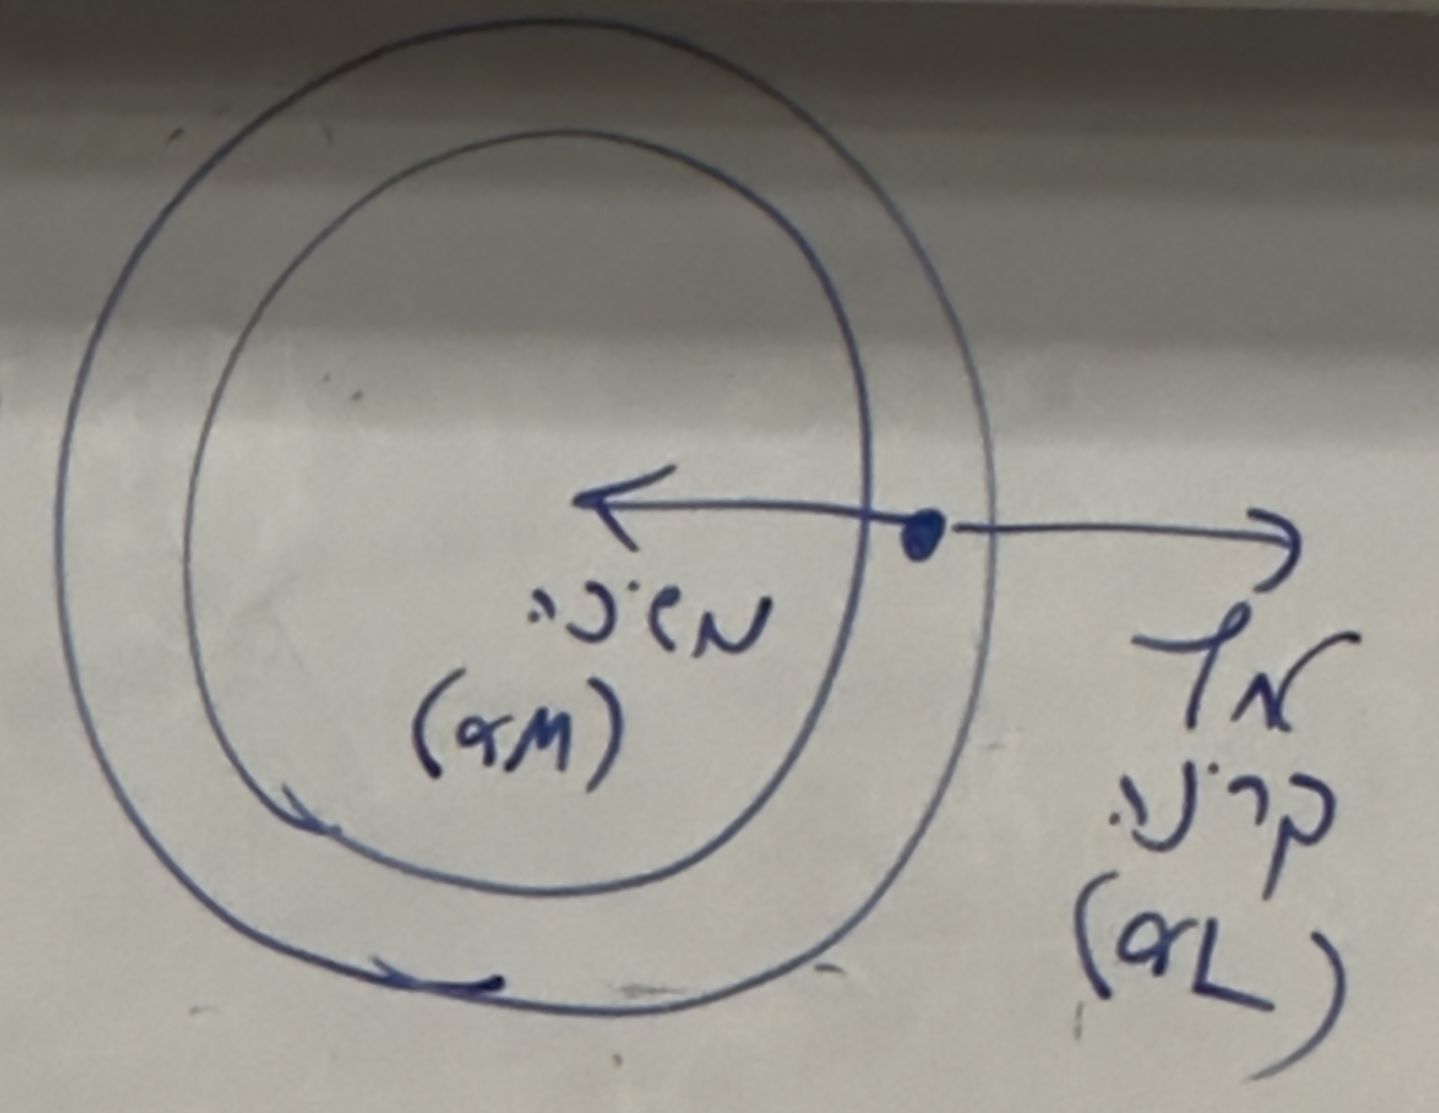
\includegraphics[width=0.5\textwidth]{images/IMG_0554.png}
\end{wrapfigure}
Let's look at the outer layer of a very massive star. Using the radiation propagation equation
\begin{equation}
	\diff{T}{r} = -\frac{3}{4ac}\frac{\kappa\rho}{T^3}\frac{L_r}{4\pi r^2c}
\end{equation}
we can rearrange it to
\begin{equation}
	\frac{1}{3}\diff*{\ins{aT^4}}{r} = -\kappa\rho\frac{L_r}{4\pi r^2c}
\end{equation}
and remembering that \(\frac{1}{3}aT^4\) is the radiation pressure
\begin{equation}
	\diff{P_{\text{rad}}}{r} = -\kappa\rho\frac{L_r}{4\pi r^2c}
\end{equation}
on the other hand, from the hydrostatic equations we have
\begin{equation}
	\diff{P}{r} = -\frac{GM_r\rho}{r^2c}
\end{equation}
setting our two expression to equal we find
\begin{equation}
	\frac{GM_r\rho}{r^2} = \kappa\rho\frac{L_r}{4\pi r^2c}
\end{equation}
isolating \(L_r\) and inserting \(r=R\)
\begin{equation}
	L_r = 4\pi c\frac{GM}{\kappa}
\end{equation}
this expression for luminosity is often called Eddington Luminosity. This expression gives us the maximum luminosity a star can have before it becomes unstable. If for a given star's parameters the observed luminosity is higher than the Eddington luminosity, then the radiation pressure will begin to overpower its hydrostatic pressure which will destabilize the star. Let's plug some numbers in to get a feel. Inserting the constants we have
\begin{equation}
	L = \SI{3.8e4}{}\frac{M}{M_\mathSun}L_\mathSun
\end{equation}
and for a mass of \(M=60M_\mathSun \)
\begin{equation}
	L = \SI{2.3e6}{L_\mathSun}
\end{equation}
\subsection{The Lifespan Of Stars}
For the Sun we can write
\begin{equation}
	t_\mathSun \simeq \frac{\eta M_{\text{core}}c^2}{L_\mathSun} \sim \SI{10}{\giga\year}
\end{equation}
If we look at stars with different masses then
\begin{equation}
	t_* \propto \frac{M}{L} \propto M^{-3} \implies t_* = t_\mathSun \ins{\frac{M}{M_\mathSun}}^{-3}
\end{equation}
\subsection{Convection}
Convection becomes important if
\begin{equation}
	t_{\text{rad}} \gg t_{\text{dyn}} = \frac{l}{c_s}
\end{equation}
\subsubsection{A more concrete criteria for convection}
Let's look at a element of gas with density \(\rho\) and temperature \(T\) at radius \(r\) in a star, which moves to \(r+dr\) and its parameters change to \(\rho+\delta\rho\) and \(T+\delta T\). The criterion for convection is
\begin{equation}
	\rho_{\text{element}}+\delta\rho_{\text{element}} < \rho_{\text{env}} + d\rho_{\text{env}}
\end{equation}
or
\begin{equation}\label{deltadrho}
	\delta\rho < d\rho
\end{equation}
then the element will float upwards. For a more accurate derivation we'l assume this is an adiabatic process, which lets us say
\begin{align}\label{deltarhooverrho}
	P\propto \rho^\gamma && \frac{\delta\rho}{\rho} = \frac{1}{\gamma}\frac{\delta P}{P} = \frac{1}{\gamma}\frac{dP}{P}
\end{align}
we'll also assume there is a pressure equilibrium with the star. Therefore
\begin{equation}
	P = \frac{\rho}{m}\kappa T
\end{equation}
which gives us
\begin{equation}\label{drhooverrho}
	\frac{d\rho}{\rho} = \frac{dP}{P}-\frac{dT}{T}
\end{equation}
We can now insert both~\ref{deltarhooverrho} and~\ref{drhooverrho} into~\ref{deltadrho} we find
\begin{equation}
	\frac{1}{\gamma}\frac{1}{P}\diff{P}{r} < \frac{1}{P}\diff{P}{r}-\frac{1}{T}\diff{T}{r}
\end{equation}
rearranging
\begin{equation}
	\diff{T}{r} < \frac{\gamma-1}{\gamma}\frac{T}{P}\diff{P}{r}
\end{equation}
both the differentials are smaller than 0, so we'll multiply both sides by \(-1\) and find
\begin{equation}\label{convection4}
	\left\lvert\diff{T}{r}\right\rvert > \frac{\gamma-1}{\gamma}\frac{T}{P}\left\lvert\diff{P}{r}\right\rvert
\end{equation}
The effect this has is that it improves the transfer of heat which in turn balances it out recursively, and after a while the greater symbol will become equal

\begin{equation}\label{convection5}
	\left\lvert\diff{T}{r}\right\rvert = \frac{\gamma-1}{\gamma}\frac{T}{P}\left\lvert\diff{P}{r}\right\rvert
\end{equation}
which is a stable state. If~\ref{convection4} is satisfied, we replace the radiation diffusion equation for the structure of stars with the convection equation~\ref{convection5}.